% Created by tikzDevice version 0.11 on 2018-05-04 09:34:17
% !TEX encoding = UTF-8 Unicode
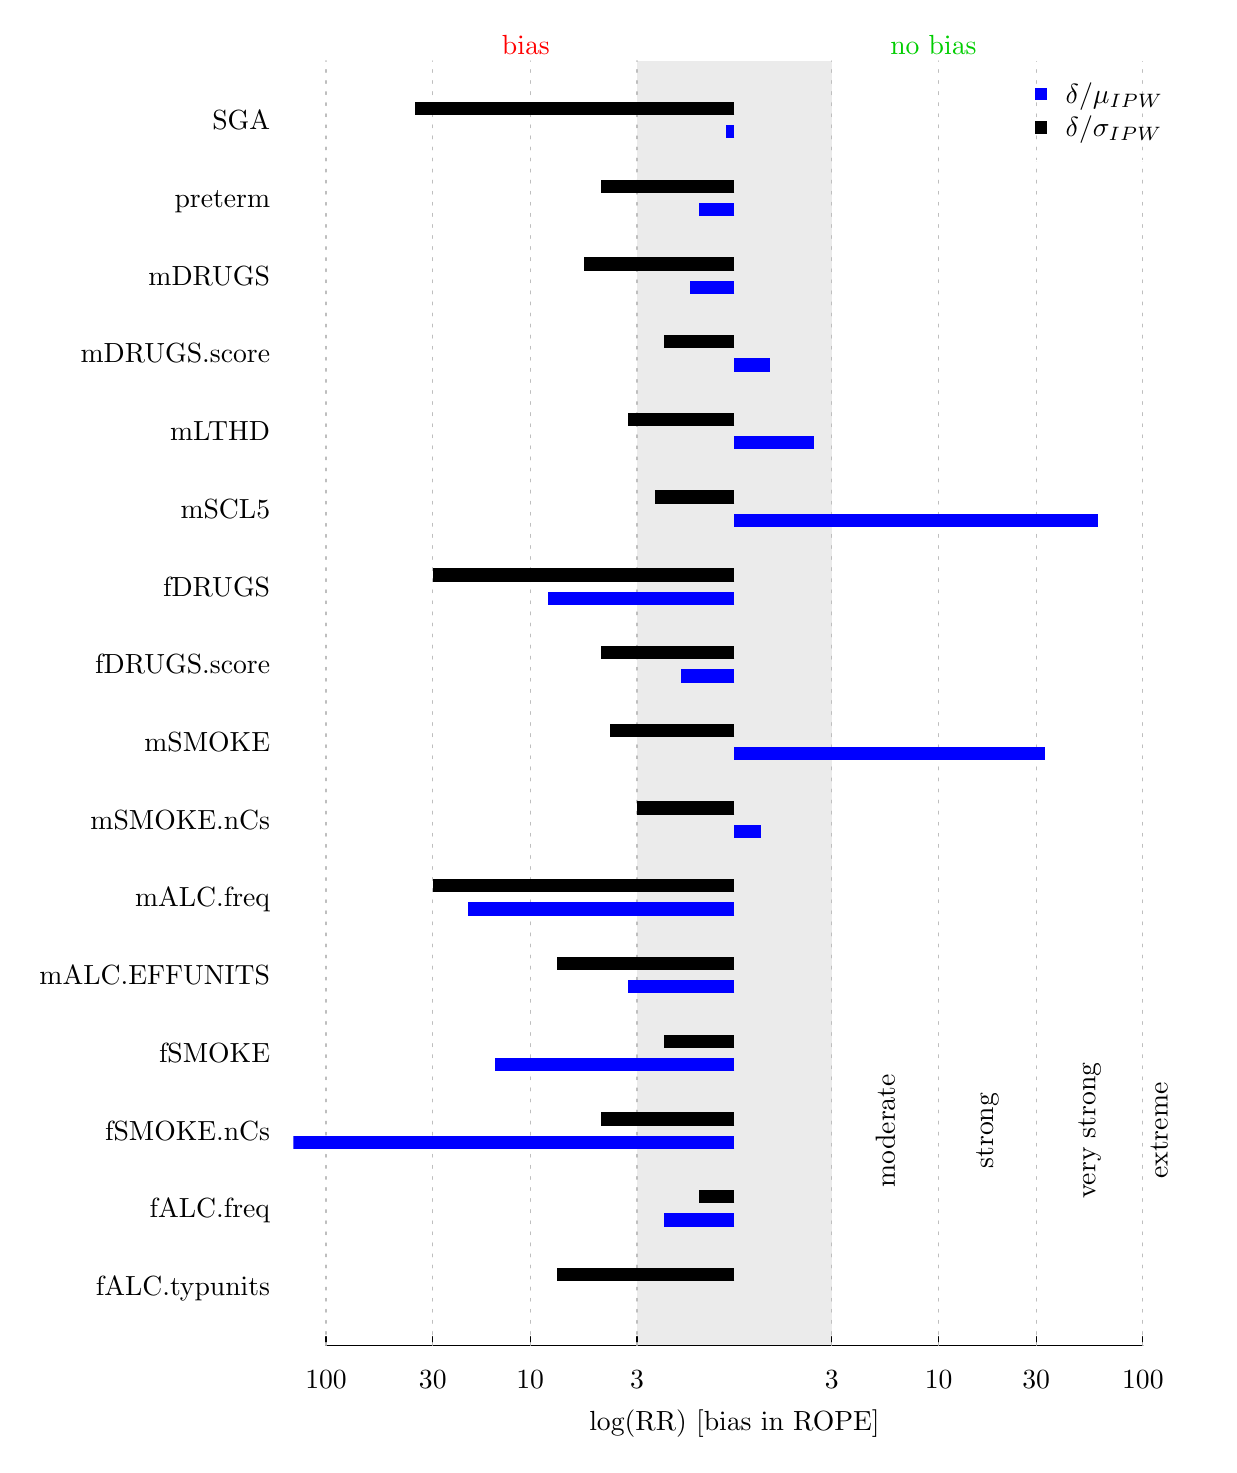
\begin{tikzpicture}[x=1pt,y=1pt]
\definecolor{fillColor}{RGB}{255,255,255}
\path[use as bounding box,fill=fillColor,fill opacity=0.00] (0,0) rectangle (426.79,512.15);
\begin{scope}
\path[clip] (  0.00,  0.00) rectangle (426.79,512.15);
\definecolor{drawColor}{RGB}{0,0,0}

\node[text=drawColor,anchor=base,inner sep=0pt, outer sep=0pt, scale=  1.00] at (255.40,  5.40) {log(RR) [bias in ROPE]};
\end{scope}
\begin{scope}
\path[clip] ( 96.00, 36.00) rectangle (414.79,500.15);
\definecolor{fillColor}{RGB}{190,190,190}

\path[fill=fillColor,fill opacity=0.30] (220.19, 36.00) rectangle (290.60,500.15);
\end{scope}
\begin{scope}
\path[clip] (  0.00,  0.00) rectangle (426.79,512.15);
\definecolor{drawColor}{RGB}{0,0,0}

\path[draw=drawColor,line width= 0.4pt,line join=round,line cap=round] (107.81, 36.00) -- (402.98, 36.00);

\path[draw=drawColor,line width= 0.4pt,line join=round,line cap=round] (107.81, 36.00) -- (107.81, 39.19);

\path[draw=drawColor,line width= 0.4pt,line join=round,line cap=round] (146.39, 36.00) -- (146.39, 39.19);

\path[draw=drawColor,line width= 0.4pt,line join=round,line cap=round] (181.60, 36.00) -- (181.60, 39.19);

\path[draw=drawColor,line width= 0.4pt,line join=round,line cap=round] (220.19, 36.00) -- (220.19, 39.19);

\path[draw=drawColor,line width= 0.4pt,line join=round,line cap=round] (290.60, 36.00) -- (290.60, 39.19);

\path[draw=drawColor,line width= 0.4pt,line join=round,line cap=round] (329.19, 36.00) -- (329.19, 39.19);

\path[draw=drawColor,line width= 0.4pt,line join=round,line cap=round] (364.40, 36.00) -- (364.40, 39.19);

\path[draw=drawColor,line width= 0.4pt,line join=round,line cap=round] (402.98, 36.00) -- (402.98, 39.19);

\node[text=drawColor,anchor=base,inner sep=0pt, outer sep=0pt, scale=  1.00] at (107.81, 20.40) {100};

\node[text=drawColor,anchor=base,inner sep=0pt, outer sep=0pt, scale=  1.00] at (146.39, 20.40) {30};

\node[text=drawColor,anchor=base,inner sep=0pt, outer sep=0pt, scale=  1.00] at (181.60, 20.40) {10};

\node[text=drawColor,anchor=base,inner sep=0pt, outer sep=0pt, scale=  1.00] at (220.19, 20.40) {3};

\node[text=drawColor,anchor=base,inner sep=0pt, outer sep=0pt, scale=  1.00] at (290.60, 20.40) {3};

\node[text=drawColor,anchor=base,inner sep=0pt, outer sep=0pt, scale=  1.00] at (329.19, 20.40) {10};

\node[text=drawColor,anchor=base,inner sep=0pt, outer sep=0pt, scale=  1.00] at (364.40, 20.40) {30};

\node[text=drawColor,anchor=base,inner sep=0pt, outer sep=0pt, scale=  1.00] at (402.98, 20.40) {100};
\end{scope}
\begin{scope}
\path[clip] ( 96.00, 36.00) rectangle (414.79,500.15);
\definecolor{drawColor}{RGB}{190,190,190}

\path[draw=drawColor,line width= 0.4pt,dash pattern=on 1pt off 3pt ,line join=round,line cap=round] (107.81, 36.00) -- (107.81,500.15);

\path[draw=drawColor,line width= 0.4pt,dash pattern=on 1pt off 3pt ,line join=round,line cap=round] (146.39, 36.00) -- (146.39,500.15);

\path[draw=drawColor,line width= 0.4pt,dash pattern=on 1pt off 3pt ,line join=round,line cap=round] (181.60, 36.00) -- (181.60,500.15);

\path[draw=drawColor,line width= 0.4pt,dash pattern=on 1pt off 3pt ,line join=round,line cap=round] (220.19, 36.00) -- (220.19,500.15);

\path[draw=drawColor,line width= 0.4pt,dash pattern=on 1pt off 3pt ,line join=round,line cap=round] (290.60, 36.00) -- (290.60,500.15);

\path[draw=drawColor,line width= 0.4pt,dash pattern=on 1pt off 3pt ,line join=round,line cap=round] (329.19, 36.00) -- (329.19,500.15);

\path[draw=drawColor,line width= 0.4pt,dash pattern=on 1pt off 3pt ,line join=round,line cap=round] (364.40, 36.00) -- (364.40,500.15);

\path[draw=drawColor,line width= 0.4pt,dash pattern=on 1pt off 3pt ,line join=round,line cap=round] (402.98, 36.00) -- (402.98,500.15);
\end{scope}
\begin{scope}
\path[clip] (  0.00,  0.00) rectangle (426.79,512.15);
\definecolor{drawColor}{RGB}{255,0,0}

\node[text=drawColor,anchor=base,inner sep=0pt, outer sep=0pt, scale=  1.00] at (180.02,502.55) {bias};
\definecolor{drawColor}{RGB}{0,205,0}

\node[text=drawColor,anchor=base east,inner sep=0pt, outer sep=0pt, scale=  1.00] at (342.88,502.55) {no bias};
\definecolor{drawColor}{RGB}{0,0,0}

\node[text=drawColor,anchor=base east,inner sep=0pt, outer sep=0pt, scale=  1.00] at ( 87.60, 53.96) {fALC.typunits};

\node[text=drawColor,anchor=base east,inner sep=0pt, outer sep=0pt, scale=  1.00] at ( 87.60, 82.05) {fALC.freq};

\node[text=drawColor,anchor=base east,inner sep=0pt, outer sep=0pt, scale=  1.00] at ( 87.60,110.14) {fSMOKE.nCs};

\node[text=drawColor,anchor=base east,inner sep=0pt, outer sep=0pt, scale=  1.00] at ( 87.60,138.23) {fSMOKE};

\node[text=drawColor,anchor=base east,inner sep=0pt, outer sep=0pt, scale=  1.00] at ( 87.60,166.32) {mALC.EFFUNITS};

\node[text=drawColor,anchor=base east,inner sep=0pt, outer sep=0pt, scale=  1.00] at ( 87.60,194.41) {mALC.freq};

\node[text=drawColor,anchor=base east,inner sep=0pt, outer sep=0pt, scale=  1.00] at ( 87.60,222.50) {mSMOKE.nCs};

\node[text=drawColor,anchor=base east,inner sep=0pt, outer sep=0pt, scale=  1.00] at ( 87.60,250.59) {mSMOKE};

\node[text=drawColor,anchor=base east,inner sep=0pt, outer sep=0pt, scale=  1.00] at ( 87.60,278.68) {fDRUGS.score};

\node[text=drawColor,anchor=base east,inner sep=0pt, outer sep=0pt, scale=  1.00] at ( 87.60,306.77) {fDRUGS};

\node[text=drawColor,anchor=base east,inner sep=0pt, outer sep=0pt, scale=  1.00] at ( 87.60,334.85) {mSCL5};

\node[text=drawColor,anchor=base east,inner sep=0pt, outer sep=0pt, scale=  1.00] at ( 87.60,362.94) {mLTHD};

\node[text=drawColor,anchor=base east,inner sep=0pt, outer sep=0pt, scale=  1.00] at ( 87.60,391.03) {mDRUGS.score};

\node[text=drawColor,anchor=base east,inner sep=0pt, outer sep=0pt, scale=  1.00] at ( 87.60,419.12) {mDRUGS};

\node[text=drawColor,anchor=base east,inner sep=0pt, outer sep=0pt, scale=  1.00] at ( 87.60,447.21) {preterm};

\node[text=drawColor,anchor=base east,inner sep=0pt, outer sep=0pt, scale=  1.00] at ( 87.60,475.30) {SGA};
\end{scope}
\begin{scope}
\path[clip] ( 96.00, 36.00) rectangle (414.79,500.15);
\definecolor{drawColor}{RGB}{0,0,255}

\path[draw=drawColor,line width= 4.8pt,line join=round] (255.40,474.53) -- (252.19,474.53);

\path[draw=drawColor,line width= 4.8pt,line join=round] (255.40,446.44) -- (242.58,446.44);

\path[draw=drawColor,line width= 4.8pt,line join=round] (255.40,418.35) -- (239.37,418.35);

\path[draw=drawColor,line width= 4.8pt,line join=round] (255.40,390.26) -- (268.22,390.26);

\path[draw=drawColor,line width= 4.8pt,line join=round] (255.40,362.17) -- (284.24,362.17);

\path[draw=drawColor,line width= 4.8pt,line join=round] (255.40,334.08) -- (386.79,334.08);

\path[draw=drawColor,line width= 4.8pt,line join=round] (255.40,306.00) -- (188.09,306.00);

\path[draw=drawColor,line width= 4.8pt,line join=round] (255.40,277.91) -- (236.17,277.91);

\path[draw=drawColor,line width= 4.8pt,line join=round] (255.40,249.82) -- (367.57,249.82);

\path[draw=drawColor,line width= 4.8pt,line join=round] (255.40,221.73) -- (265.01,221.73);

\path[draw=drawColor,line width= 4.8pt,line join=round] (255.40,193.64) -- (159.25,193.64);

\path[draw=drawColor,line width= 4.8pt,line join=round] (255.40,165.55) -- (216.94,165.55);

\path[draw=drawColor,line width= 4.8pt,line join=round] (255.40,137.46) -- (168.86,137.46);

\path[draw=drawColor,line width= 4.8pt,line join=round] (255.40,109.37) -- ( 72.72,109.37);

\path[draw=drawColor,line width= 4.8pt,line join=round] (255.40, 81.28) -- (229.76, 81.28);

\path[draw=drawColor,line width= 4.8pt,line join=round] (255.40, 53.19) -- (255.40, 53.19);
\definecolor{drawColor}{RGB}{0,0,0}

\path[draw=drawColor,line width= 4.8pt,line join=round] (255.40,482.96) -- (140.02,482.96);

\path[draw=drawColor,line width= 4.8pt,line join=round] (255.40,454.87) -- (207.32,454.87);

\path[draw=drawColor,line width= 4.8pt,line join=round] (255.40,426.78) -- (200.91,426.78);

\path[draw=drawColor,line width= 4.8pt,line join=round] (255.40,398.69) -- (229.76,398.69);

\path[draw=drawColor,line width= 4.8pt,line join=round] (255.40,370.60) -- (216.94,370.60);

\path[draw=drawColor,line width= 4.8pt,line join=round] (255.40,342.51) -- (226.55,342.51);

\path[draw=drawColor,line width= 4.8pt,line join=round] (255.40,314.42) -- (146.43,314.42);

\path[draw=drawColor,line width= 4.8pt,line join=round] (255.40,286.33) -- (207.32,286.33);

\path[draw=drawColor,line width= 4.8pt,line join=round] (255.40,258.24) -- (210.53,258.24);

\path[draw=drawColor,line width= 4.8pt,line join=round] (255.40,230.15) -- (220.14,230.15);

\path[draw=drawColor,line width= 4.8pt,line join=round] (255.40,202.06) -- (146.43,202.06);

\path[draw=drawColor,line width= 4.8pt,line join=round] (255.40,173.98) -- (191.30,173.98);

\path[draw=drawColor,line width= 4.8pt,line join=round] (255.40,145.89) -- (229.76,145.89);

\path[draw=drawColor,line width= 4.8pt,line join=round] (255.40,117.80) -- (207.32,117.80);

\path[draw=drawColor,line width= 4.8pt,line join=round] (255.40, 89.71) -- (242.58, 89.71);

\path[draw=drawColor,line width= 4.8pt,line join=round] (255.40, 61.62) -- (191.30, 61.62);
\end{scope}
\begin{scope}
\path[clip] (  0.00,  0.00) rectangle (426.79,512.15);
\definecolor{drawColor}{RGB}{0,0,0}

\node[text=drawColor,rotate= 90.00,anchor=base,inner sep=0pt, outer sep=0pt, scale=  1.00] at (313.34,113.58) {moderate};

\node[text=drawColor,rotate= 90.00,anchor=base,inner sep=0pt, outer sep=0pt, scale=  1.00] at (348.90,113.58) {strong};

\node[text=drawColor,rotate= 90.00,anchor=base,inner sep=0pt, outer sep=0pt, scale=  1.00] at (385.79,113.58) {very strong};

\node[text=drawColor,rotate= 90.00,anchor=base,inner sep=0pt, outer sep=0pt, scale=  1.00] at (411.96,113.58) {extreme};
\definecolor{drawColor}{RGB}{255,255,255}

\path[draw=drawColor,line width= 0.4pt,line join=round,line cap=round] (357.09,500.15) rectangle (414.79,464.15);
\definecolor{fillColor}{RGB}{0,0,255}

\path[fill=fillColor] (363.84,485.90) --
	(368.34,485.90) --
	(368.34,490.40) --
	(363.84,490.40) --
	cycle;
\definecolor{fillColor}{RGB}{0,0,0}

\path[fill=fillColor] (363.84,473.90) --
	(368.34,473.90) --
	(368.34,478.40) --
	(363.84,478.40) --
	cycle;
\definecolor{drawColor}{RGB}{0,0,0}

\node[text=drawColor,anchor=base west,inner sep=0pt, outer sep=0pt, scale=  1.00] at (375.09,484.71) {$\delta/\mu_{IPW}$};

\node[text=drawColor,anchor=base west,inner sep=0pt, outer sep=0pt, scale=  1.00] at (375.09,472.71) {$\delta/\sigma_{IPW}$};
\end{scope}
\end{tikzpicture}
